\documentclass{beamer}
 
\usepackage[utf8]{inputenc}
\usetheme{Madrid}

\usepackage{biblatex}

\usepackage{mathrsfs}

\DeclareMathOperator*{\argmin}{arg\,min}


\newcommand*{\TitleFont}{%
      \usefont{\encodingdefault}{\rmdefault}{b}{n}%
      \fontsize{9}{20}%
      \selectfont}
      
    
%\renewcommand{\figurename}{Fig.}  

\usepackage[figurename=]{caption}

\newsavebox{\authbox}
\sbox{\authbox}{%
\centering
\begin{minipage}{0.33\linewidth}
\centering\normalsize
Candidate \par
Rodrigo Ramele
\end{minipage}
\hfill
\begin{minipage}{0.33\linewidth}
\centering\normalsize
Supervisor \par
Dr. Juan Miguel Santos
\end{minipage}

\begin{minipage}{0.33\linewidth}
\centering\normalsize
Cosupervisor \par
Dra. Ana Julia Villar
\end{minipage}
}
 
%Information to be included in the title page:
\title[HIST of EEG for BCI] %optional
{Histogram of Gradient Orientations of EEG Signal Plots for Brain Computer Interfaces}
 
\subtitle{Thesis}
 
\author[Ramele, Rodrigo]{ % (optional, for multiple authors)
\usebox{\authbox}
}
 
\institute[ITBA] % (optional)
{
  Doctorado en Ingeniería en Informática\\
  Instituto Tecnológico de Buenos Aires
}
 
\date[Nov 29, 2018] % (optional)
{Noviembre 29 2018}
 
\logo{
\includegraphics[height=1.0cm]{images/itbalogo.png}}
 
 
 
\begin{document}
 
\frame{\titlepage}
 
\begin{frame}
\frametitle{Sample frame title}
This is a text in first frame. This is a text in first frame. This is a text in first frame.
\end{frame}
 
\begin{frame}
\frametitle{Table of Contents}
\tableofcontents
\end{frame} 

\begin{frame}
\frametitle{Sample frame title}
This is a text in second frame. 
For the sake of showing an example.
 
\begin{itemize}
 \item<1-> Text visible on slide 1
 \item<2-> Text visible on slide 2
 \item<3> Text visible on slide 3
 \item<4-> Text visible on slide 4
\end{itemize}
 
\end{frame}

\begin{frame}
\frametitle{Sample frame title}
\begin{equation}
 \omega_\mathrm{ang}(\alpha) = \sum_{r=-1}^{1} \omega \bigg ( \frac{8\alpha}{2\pi} + 8r \bigg )
\label{eq:wang}
\end{equation}
\end{frame}

\begin{frame}
\frametitle{Sample frame title}
 
In this slide, some important text will be
\alert{highlighted} beause it's important.
Please, don't abuse it.
 
\begin{block}{Remark}
Sample text
\end{block}
 
\begin{alertblock}{Important theorem}
Sample text in red box
\end{alertblock}
 
\begin{examples}
Sample text in green box. "Examples" is fixed as block title.
\end{examples}
\end{frame}



\begin{frame}
\frametitle{Alpha Waves wiggles}


\end{frame}

\begin{frame}
\frametitle{Mu a Greek letter}


\end{frame}


\begin{frame}
\frametitle{The P300 Wave}


\end{frame}


	\begin{frame}
		\begin{center}
  		
\includegraphics[scale=0.05]{images/itba.pdf}		
		\end{center}
  		\titlepage
	\end{frame}

    \begin{frame}
        \frametitle{Outline}
        \tableofcontents{}
    \end{frame}
    
    
    \section{Introduction}
    \begin{frame}
        \frametitle{Introduction}
        \begin{center}
            \begin{itemize}
                \item BCI challenging technology.
                \item Outstanding advances but yet its push into mainstream technology has not fully materialized.
                \item More clinical and physician Involvement: devise mechanisms to help them stay in the loop.
            \end{itemize}
        \end{center}
    \end{frame}
    
    
    \section{Motivation}
    \begin{frame}
        \frametitle{Motivation}
        \begin{center}
            \begin{itemize}
                \item Is it possible to discriminate EEG signals and their corresponding cognitive processes based on their plots? 
                \item Are those visual wiggles simple noise or can we extract something meaningful from them ?
            \end{itemize}
        \end{center}
    \end{frame}
    \begin{frame}
        \frametitle{What we aim to do}
        \begin{center}
            \begin{itemize}
                \item Establish a Fruitful connection between Image Processing and EEG Analysis
                \item Provide a Framework to analyze visually relevant features from EEG.
                \item Assess the method by performing Binary Classification on known datasets.
            \end{itemize}
        \end{center}
    \end{frame}
    
    
   \section{Method}
   \section{Offline Results}
    \begin{frame}
        \begin{center}
            \LARGE Method   
        \end{center}
    \end{frame}
    
    \subsection{Signal Transformation}
    \begin{frame}
        \frametitle{Signal Transformation}
        \begin{center}           

Single Channel transformation of the EEG multichannel time series matrix into an image
\begin{equation}
\mathscr{T}\{x(t,c,V)=0\} \mapsto I(z_1,z_2, \mathcal{C}, \mathcal{I}) = 0
\end{equation}
where $ t $ is time, $ c $ is the specified channel, $ V $ is the voltage value for the signal, $ \mathcal{C} $ is the color channel for an image and  $ \mathcal{I} $ is the pixel value intensity.

\vspace{17pt}

Plot Generation: The EEG matrix is transformed to a binary bidimensional image $ (t,c,V) \mapsto (t, V, Grey, \mathcal{I}) $ with $\mathcal{I} = 0$ or  $\mathcal{I} = 255$ for each $ c $.

		\end{center}
	\end{frame}
	
	\begin{frame}
	\frametitle{Signal Transformation: Visually centering the signal over the image.}
	\begin{center}

First the non-zero media is removed from the signal.
	
\begin{equation}
\tilde{x}(t,c) = \lfloor  \delta .(  x(t,c) - \bar{x}(c)  )   \rfloor 
\end{equation}
	
And the signal is centered on the image

\begin{equation}
h(c) = ( \max{} \tilde{x}(t,c) - \min{} \tilde{x}(t,c) ) + \sigma 
\end{equation}

\begin{equation}
Z(c) = \lfloor \frac{h(c)}{2} \rfloor - \lfloor \frac{\max{} \tilde{x}(t,c) + \min{} \tilde{x}(t,c)}{2} \rfloor 
\end{equation}

where $ t $ is time, $ \delta $ is scale factor,  $ c $ is the channel parameter, $ x(t,c) $ is the EEG matrix whereas $ \bar{x}(c) $ is the mean value for each channel,  $ h(c) $ is the height of the image in pixels, $ \sigma $ is the descriptor size and $ Z(c) $ is the horizontal pixel at which the zero value of the signal will be located.

	\end{center}
	\end{frame}

	\begin{frame}
	\frametitle{Signal Transformation: Binary Image generation.}
	\begin{center}
	
\begin{equation}
I(z_1,z_2) = \left\{ \begin{array}{rl}
255      & z_1 = \delta \cdot t;  z_2 = \tilde{x}(t,c) + Z(c)   \\
0   & \mbox{otherwise}
\end{array}\right. 
\end{equation}

		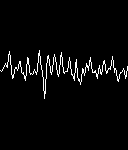
\includegraphics[scale=2]{images/SignalSample.png} 
		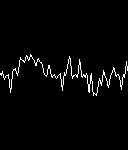
\includegraphics[scale=2]{images/SignalSample2.png} 
		
% \eqno{(2)}

        \end{center}
    \end{frame}


%    \begin{frame}
  %      \frametitle{Signal Transformation}
 %       \begin{center}           
   %     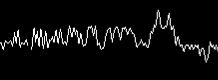
\includegraphics[scale=4]{images/SignalTransformation.png} 
     %   \end{center}
    %\end{frame}
    
    \subsection{Feature Extraction}
    \begin{frame}
    \frametitle{Features: SIFT\footfullcite{Lowe 2004} Descriptors}
    
    Scale Invariant Feature Transform Descriptors are local features of an image that represents gradient changes in intensities.  They are 128-dimensional vectors that contains the histograms of relative gradient directions on each of the blocks that each patch is divided (4x4=16 blocks, 8 rotational directions on each).  A single scale ($ \sigma = 1 $) is composed of 4 blocks of 3 pixels on each side (12x12).
    
        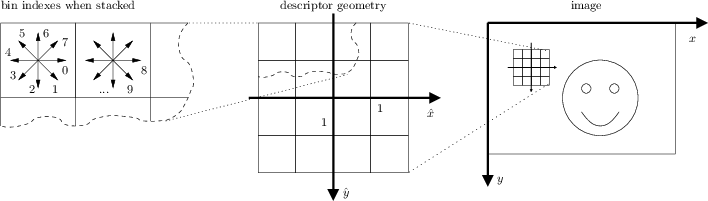
\includegraphics[scale=0.5]{images/sift-conv-vlfeat.png}     
    \end{frame}
    
    \begin{frame}
        \frametitle{SIFT Descriptors}
        \begin{center}
   			\begin{figure}[thpb]
      			\centering
      			\setlength\fboxsep{0pt}
	  			\setlength\fboxrule{0.5pt}
       			\fbox{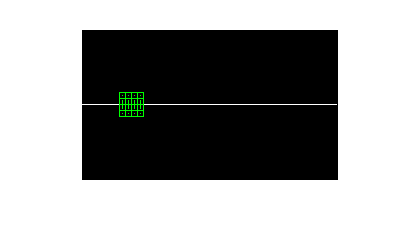
\includegraphics[scale=0.7]{images/BaselineDescriptor.png}}
      			\caption{\centering SIFT Descriptor $ [ z_1, z_2, \theta, \sigma ] $ where $ (z_1, z_2) $ are the 2D coordinates where the \textit{Keypoint} is located, $ \theta $ is the descriptor general orientation and $ \sigma $ is the descriptor size. }
      			\label{figure1}
   			\end{figure}        
        \end{center}
    \end{frame}   
    
    \begin{frame}
        \frametitle{SIFT Descriptors}
        \begin{center}
   			\begin{figure}[thpb]
      		\centering
      		\setlength\fboxsep{0pt}
	  		\setlength\fboxrule{0.5pt}
       		\fbox{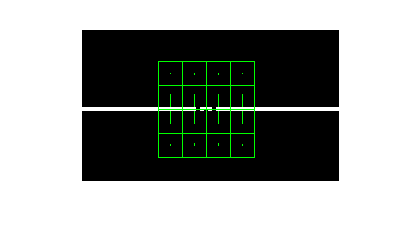
\includegraphics[scale=0.8]{images/BaselineDescriptorZoom.png}}
      		\caption{\centering  SIFT Descriptor with its corresponding gradient tendencies.}
      		\label{figure1}
   			\end{figure}        
        \end{center}
    \end{frame}   
    
    \begin{frame}
        \frametitle{SIFT Descriptors}
        \begin{center}
   			\begin{figure}[thpb]
      		\centering
      		\setlength\fboxsep{0pt}
	  		\setlength\fboxrule{0.5pt}
       		\fbox{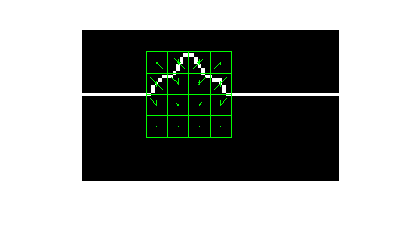
\includegraphics[scale=0.6]{images/EasyDescriptorSample1.png}}
       		\fbox{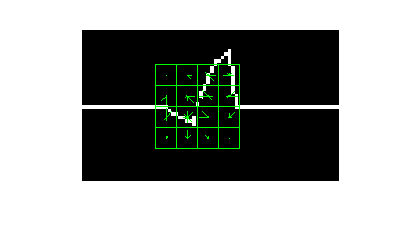
\includegraphics[scale=0.6]{images/EasyDescriptorSample2.png}}
      		\caption{\centering Sample Descriptors from artificial signals.}
      		\label{figure1}
   			\end{figure}        
        \end{center}
    \end{frame}       
        
    \begin{frame}
        \frametitle{SIFT Descriptors}
        \begin{center}
   			\begin{figure}[thpb]
      		\centering
      		\setlength\fboxsep{0pt}
	  		\setlength\fboxrule{0.5pt}
       		\fbox{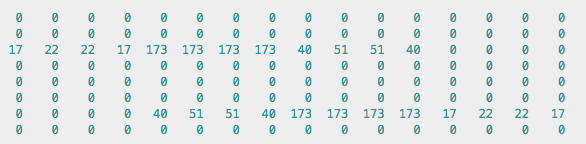
\includegraphics[scale=0.48]{images/BaselineDescriptorValues2.png}}
      		\caption{\centering Sample descriptor values of the given patch.}
      		\label{figure1}
   			\end{figure}        
        \end{center}
    \end{frame}   
    
    %\begin{frame}
     %   \frametitle{SIFT Descriptors}
       % \begin{center}
   		%	\begin{figure}[thpb]
      	%		\centering
      	%		\setlength\fboxsep{0pt}
	  	%		\setlength\fboxrule{0.5pt}
       	%		\fbox{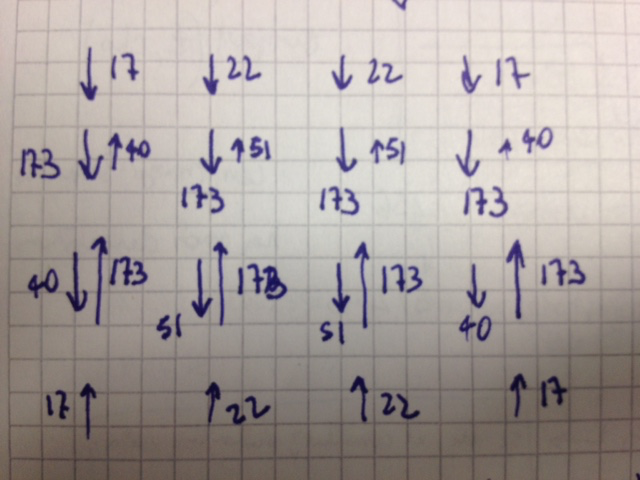
\includegraphics[scale=0.4]{images/BaselineDescriptorRepresentation.png}}
      	%		\caption{\centering Descriptor values and their representation as intensity gradients.}
      	%		\label{figure1}
   		%	\end{figure}        
       % \end{center}
    %\end{frame}   
    
    \begin{frame}
        \frametitle{Keypoint Localization}
        \begin{center}
   			\begin{figure}[thpb]
      			\centering
      			\setlength\fboxsep{0pt}
	  			\setlength\fboxrule{0.5pt}
       			%\fbox{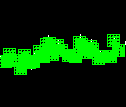
\includegraphics[scale=1.5]{images/KeypointLocations2.png}}
       			\fbox{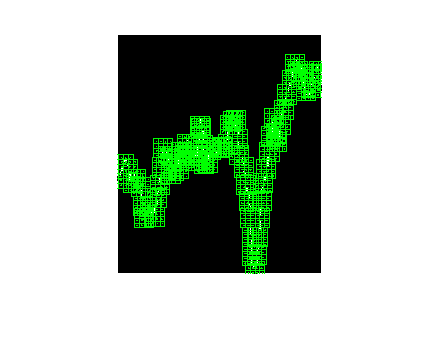
\includegraphics[scale=0.58]{images/SignalWithFullDescriptors.png}}
      			\caption{\centering Keypoints are $ (z_1, z_2) $ points on the image where descriptors are extracted.}
      			\label{figure1}
   			\end{figure}        
        \end{center}
    \end{frame}      
     
     
    
    \subsection{Classification}
    \begin{frame}
        \frametitle{Classification}
        \begin{center}
            \begin{itemize}
                \item Discriminative Semi-supervised classification method was used:  Naive Bayes Nearest Neighbor, NBNN\footfullcite{Boiman, Shechtman, Irani 2008} algorithm:
			\end{itemize}
                
                
$$
\hat{C} = \argmin_C \sum {\lVert  d_i - NN_C(d_i)  \rVert}^2 \eqno{(3)}
$$                 
   
where $ \hat{C} $ is estimated Class to which this image (and underlying EEG signal windows) should belong whereas $ d_i $ is the i-th descriptor obtained from the query image and  $ NN_C(d_i)  $ is the near neighbor descriptor for each class.         
                
        \end{center}
    \end{frame}
    
    % Graph NBNN
    \begin{frame}
        \frametitle{Classification}
        \begin{center}
            \item 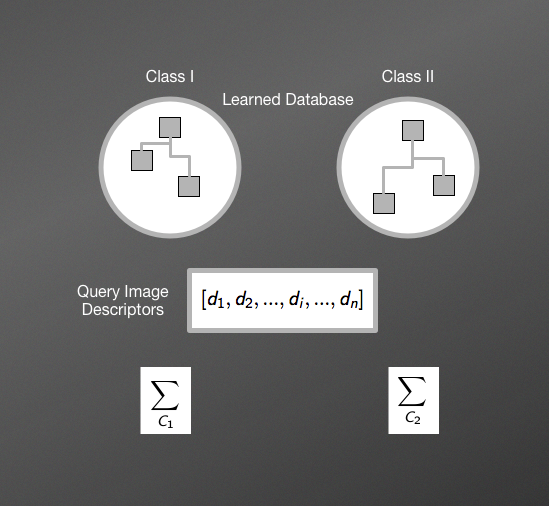
\includegraphics[scale=0.38]{images/NBNNMethod1.png}     
        \end{center}
    \end{frame}
    
    \begin{frame}
        \frametitle{Classification}
        \begin{center}
            \item 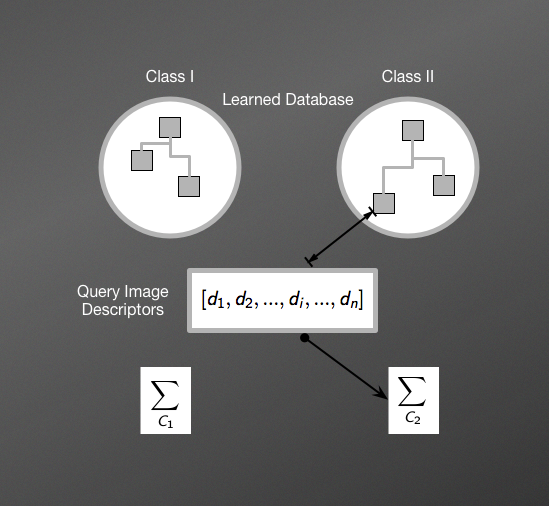
\includegraphics[scale=0.38]{images/NBNNMethod2.png}        
        \end{center}
    \end{frame}
    
    \begin{frame}
        \frametitle{Classification}
        \begin{center}
            \item 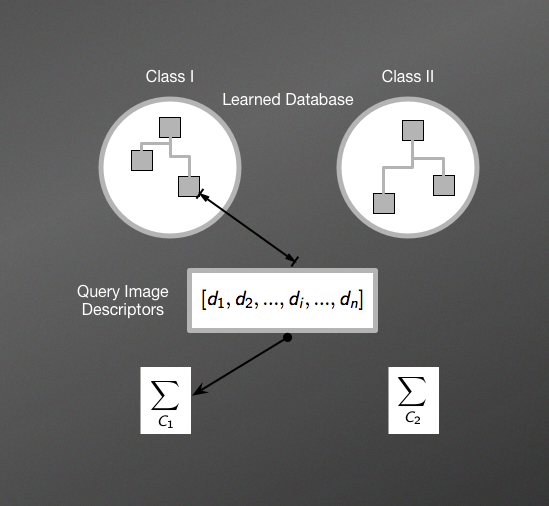
\includegraphics[scale=0.38]{images/NBNNMethod3.png}    
        \end{center}
    \end{frame}    

    \begin{frame}
        \frametitle{Classification}
        \begin{center}
            \item 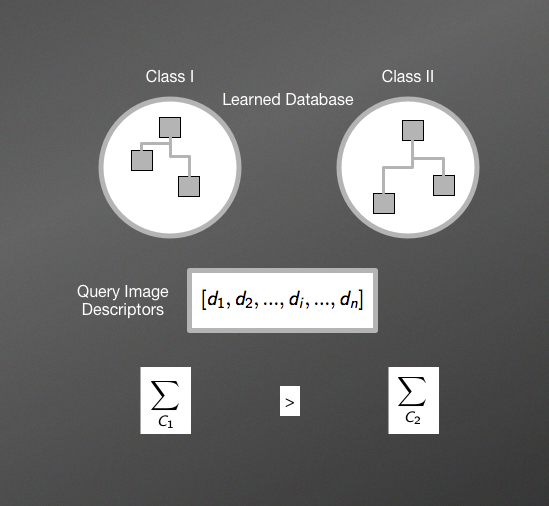
\includegraphics[scale=0.38]{images/NBNNMethod4.png}     
        \end{center}
    \end{frame}    
    
    \begin{frame}
        \frametitle{Classification}
        \begin{center}
            \item 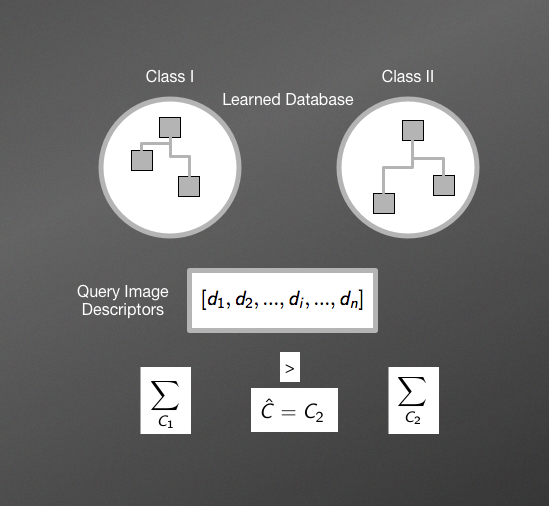
\includegraphics[scale=0.38]{images/NBNNMethod5.png}     
        \end{center}
    \end{frame}    
    
    
    \section{Offline Results}
    \begin{frame}
        \begin{center}
            \LARGE Offline Results   
        \end{center}
    \end{frame}
    
    \subsection{Inter-Subject Occipital Alpha Waves}
    \begin{frame}
        \frametitle{Dataset I: Subject Independent $\alpha $ Waves \footfullcite{Ramele, Villar, Santos 2014}}        
   \begin{figure}[thpb]
      \centering
      \setlength\fboxsep{0pt}
	  \setlength\fboxrule{0.5pt}
       \fbox{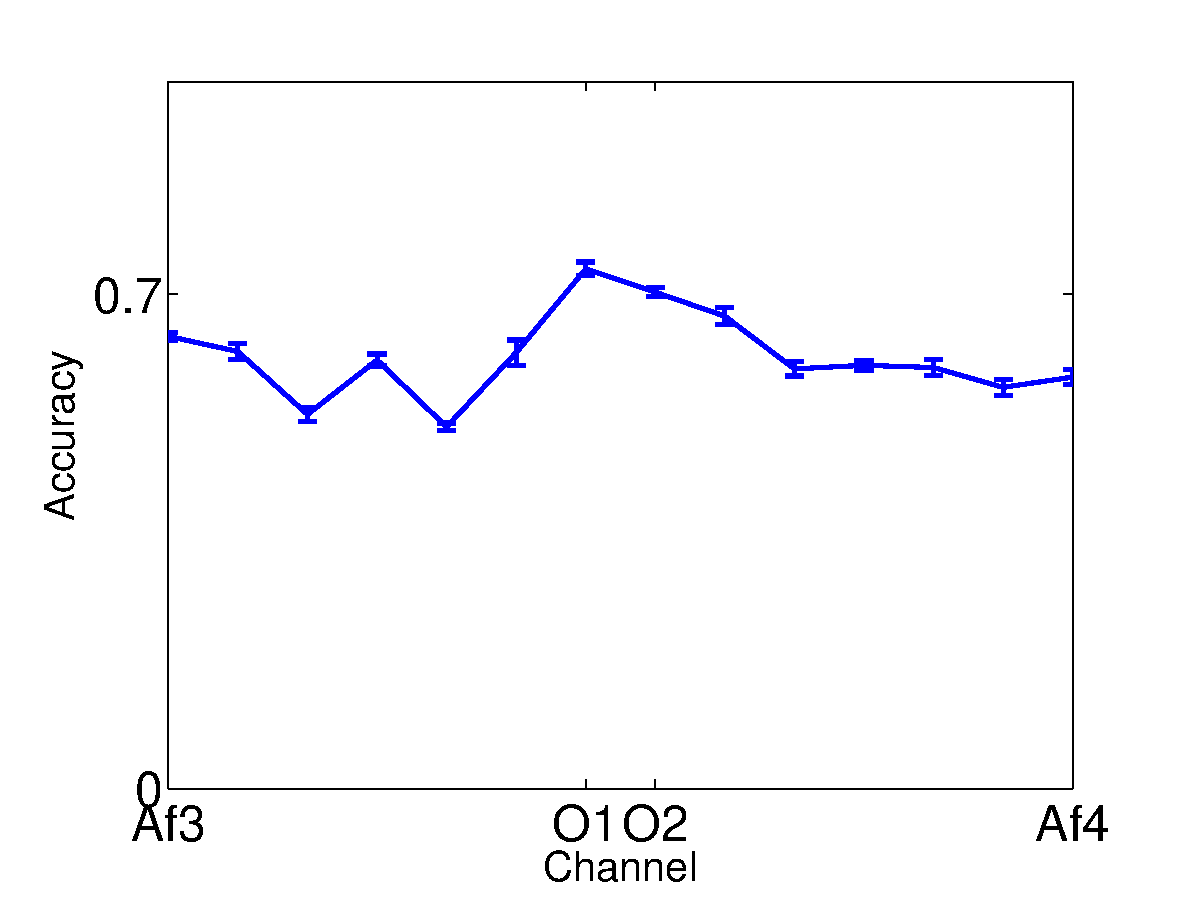
\includegraphics[scale=0.46]{images/Dataset1AccuracyPerChannel.eps}}
      \caption{\centering 10-Fold Cross validated accuracy values for 10 subjects.}
      \label{figure2}
   \end{figure}   
    \end{frame}
    
    
    \subsection{Physiobank EEG Dataset, Runs 1 and 2}
    \begin{frame}
      \frametitle{Dataset II: EEG Dataset, Runs 1 and 2 \footfullcite{Goldberg et al 2000, Schalk 2004}}
   \begin{figure}[thpb]
      \centering
      \setlength\fboxsep{0pt}
	  \setlength\fboxrule{0.5pt}
       \fbox{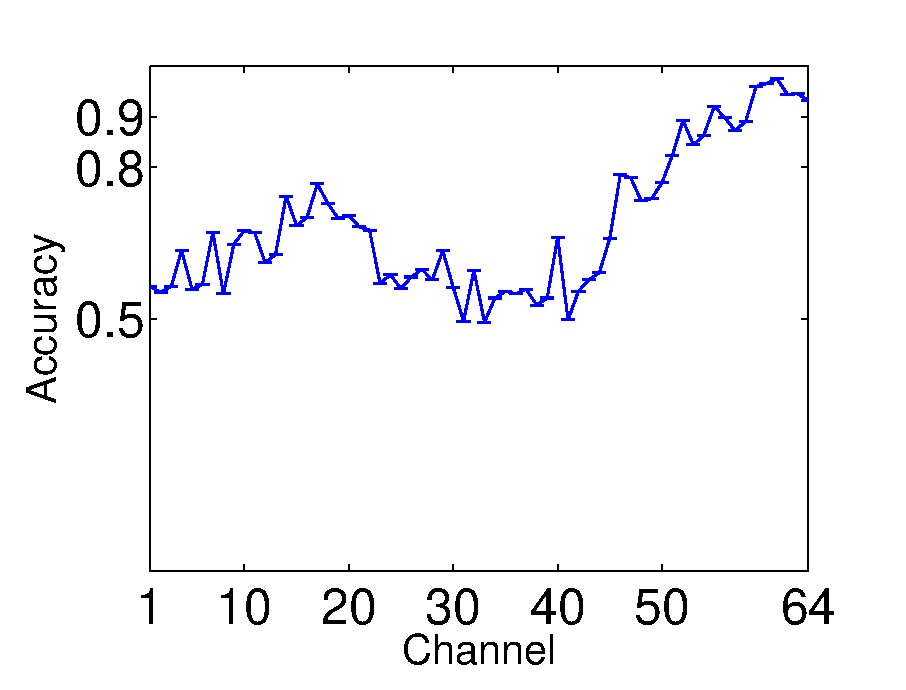
\includegraphics[scale=0.58]{images/DatasetPhysionetAccuracyPerChannel}}
      \caption{\centering 10-Fold Cross validated accuracies values for one random subject.}
      \label{figure2}
   \end{figure}          
    \end{frame}    

    \begin{frame}
    \frametitle{Dataset II: EEG Dataset, Runs 1 and 2 \footfullcite{Goldberg et al 2000, Schalk 2004}}
   \begin{figure}[thpb]
      \centering
      \setlength\fboxsep{0pt}
	  \setlength\fboxrule{0.5pt}
       \fbox{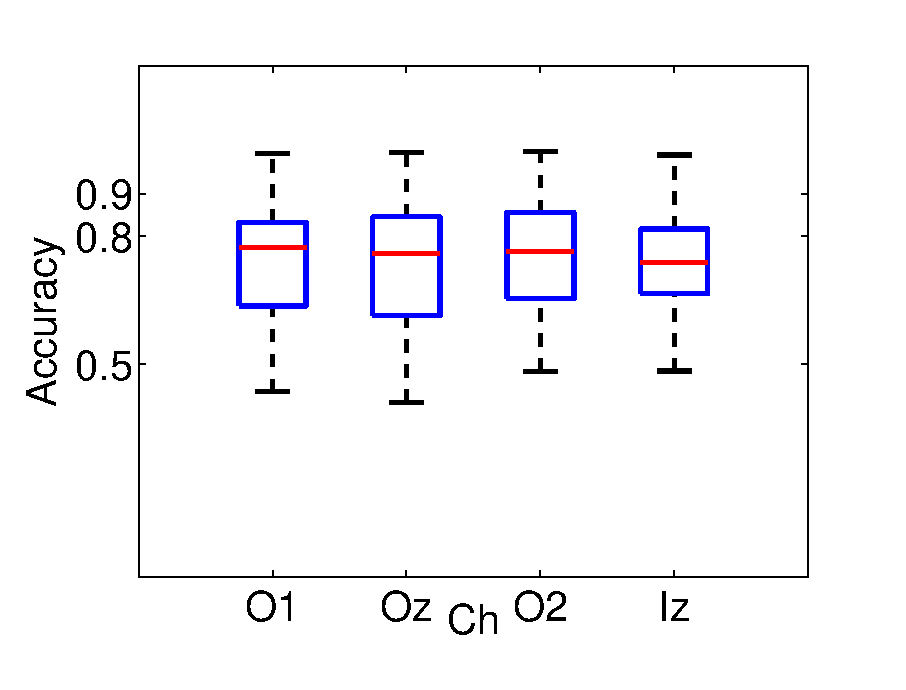
\includegraphics[scale=0.63]{images/DatasetPhysionetBoxPlots}}
      \caption{\centering 10-Fold Cross validated accuracies for O1, Oz, O2 and Iz channels for 25 subjects.}
      \label{figure2}
   \end{figure}          
    \end{frame}            
        
   %\begin{frame}     
   %\begin{figure}[thpb]
    %  \centering
    %  \setlength\fboxsep{0pt}
	 % \setlength\fboxrule{0.5pt}
     %  \fbox{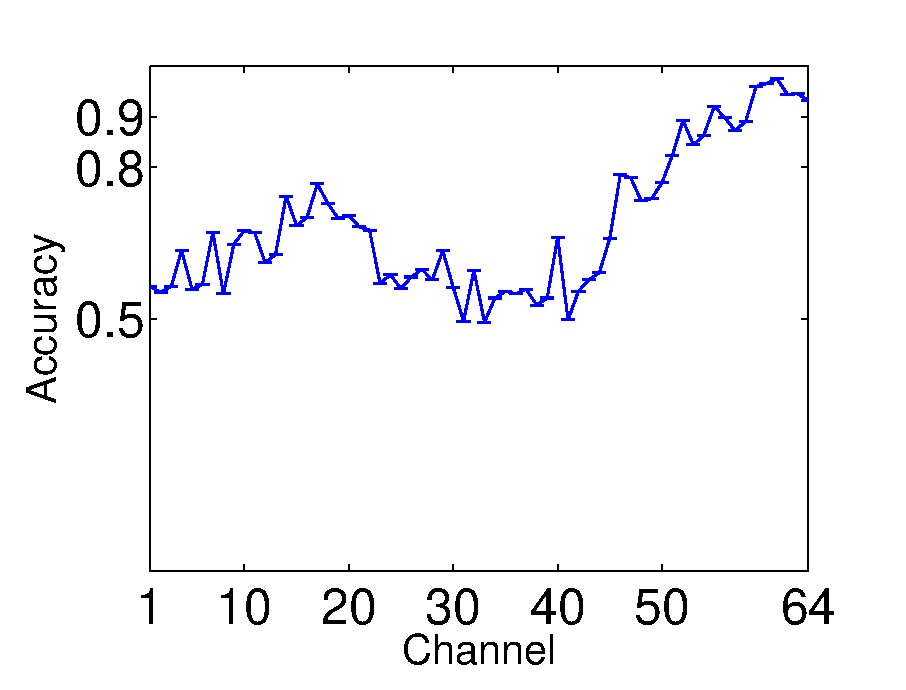
\includegraphics[scale=0.3]{images/DatasetPhysionetAccuracyPerChannel}}
     %  \fbox{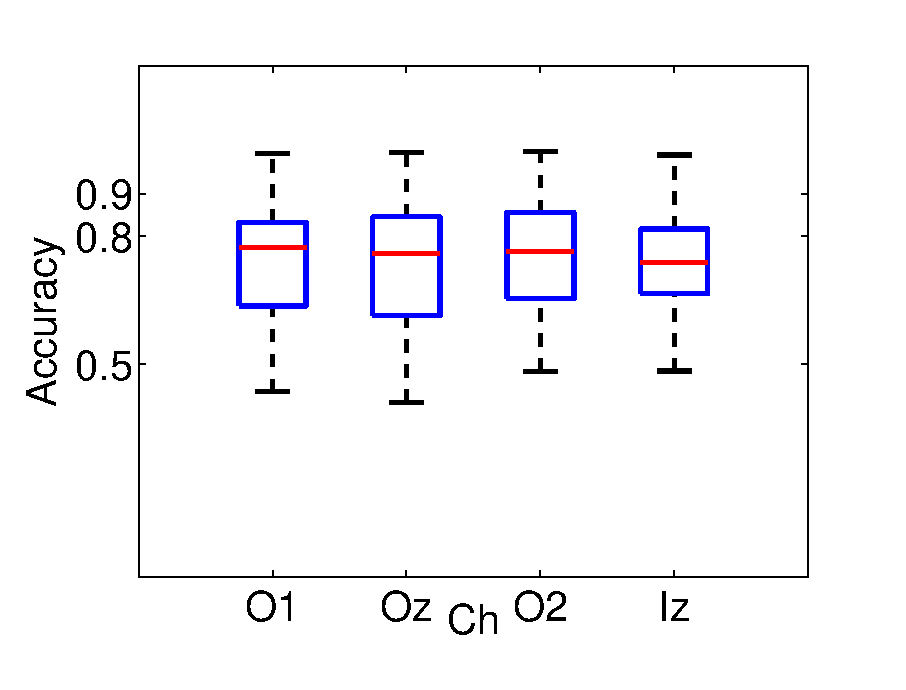
\includegraphics[scale=0.3]{images/DatasetPhysionetBoxPlots}}
     % \caption{10-KFold CrossValidation}
     % \label{figure2}
   %\end{figure}  
    %\end{frame}
    
    
    \subsection{Motor Imagery (BNCI Horizon 2020 Dataset 002-2014)} 	
	\begin{frame}
	  \frametitle{Dataset III: Motor Imagery \footfullcite{Steyrl, Scherer et al 2015}}
       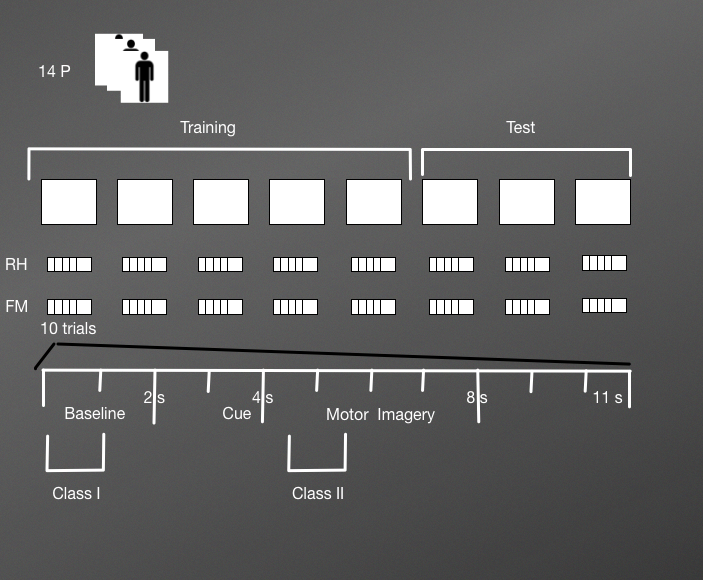
\includegraphics[scale=0.38]{images/DatasetIIIDiagram2}    
    \end{frame}
   
   
   \begin{frame}   
   \begin{figure}[thpb]
      \centering
      \setlength\fboxsep{0pt}
	  \setlength\fboxrule{0.5pt}
       \fbox{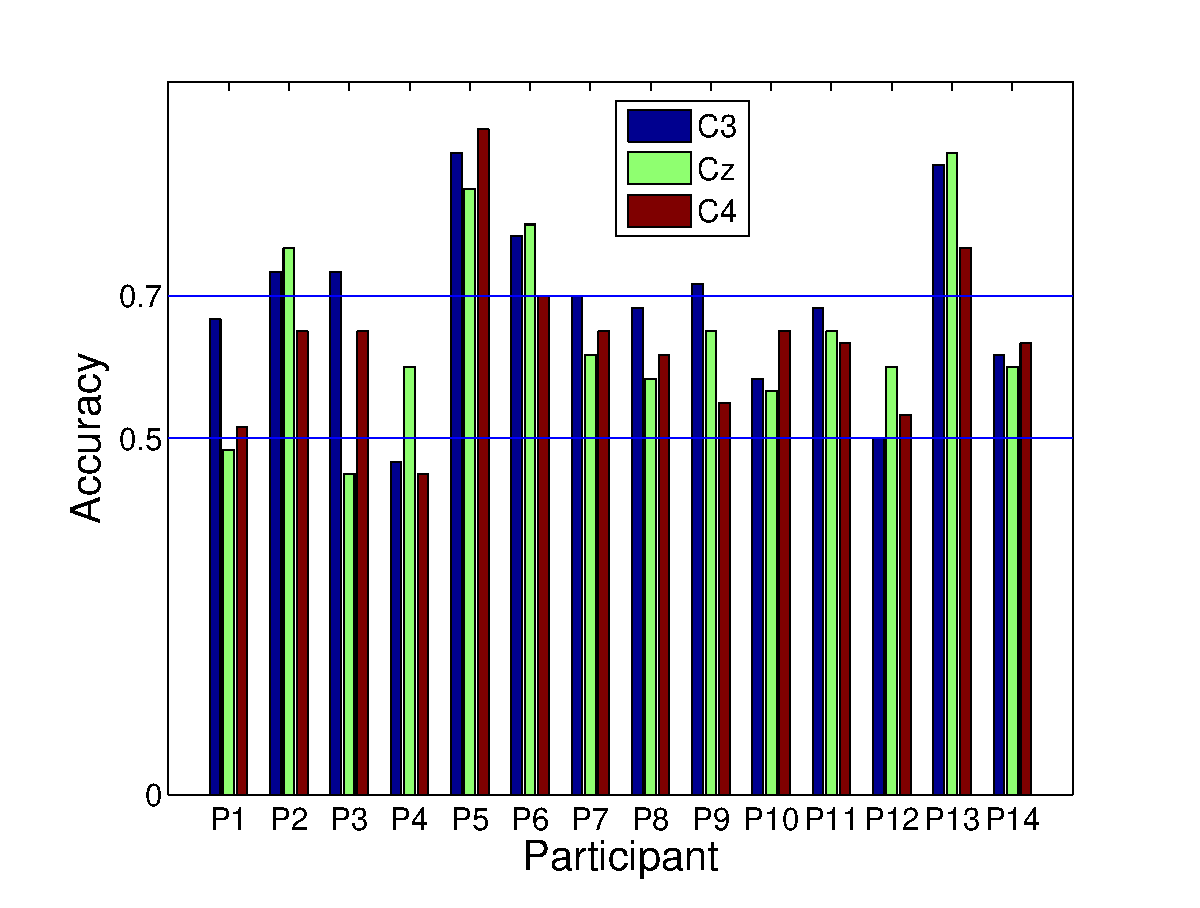
\includegraphics[scale=0.45]{images/DatasetMIBCISimulation1}}
      \caption{\centering Accuracy for the BCI Simulation classifying Baseline vs. RH (Right Hand) motor imagery.}
      \label{figure3}
   \end{figure} 	
	\end{frame}	  
	
	
	\begin{frame}
   \begin{figure}[thpb]
      \centering
      \setlength\fboxsep{0pt}
	  \setlength\fboxrule{0.5pt}
       \fbox{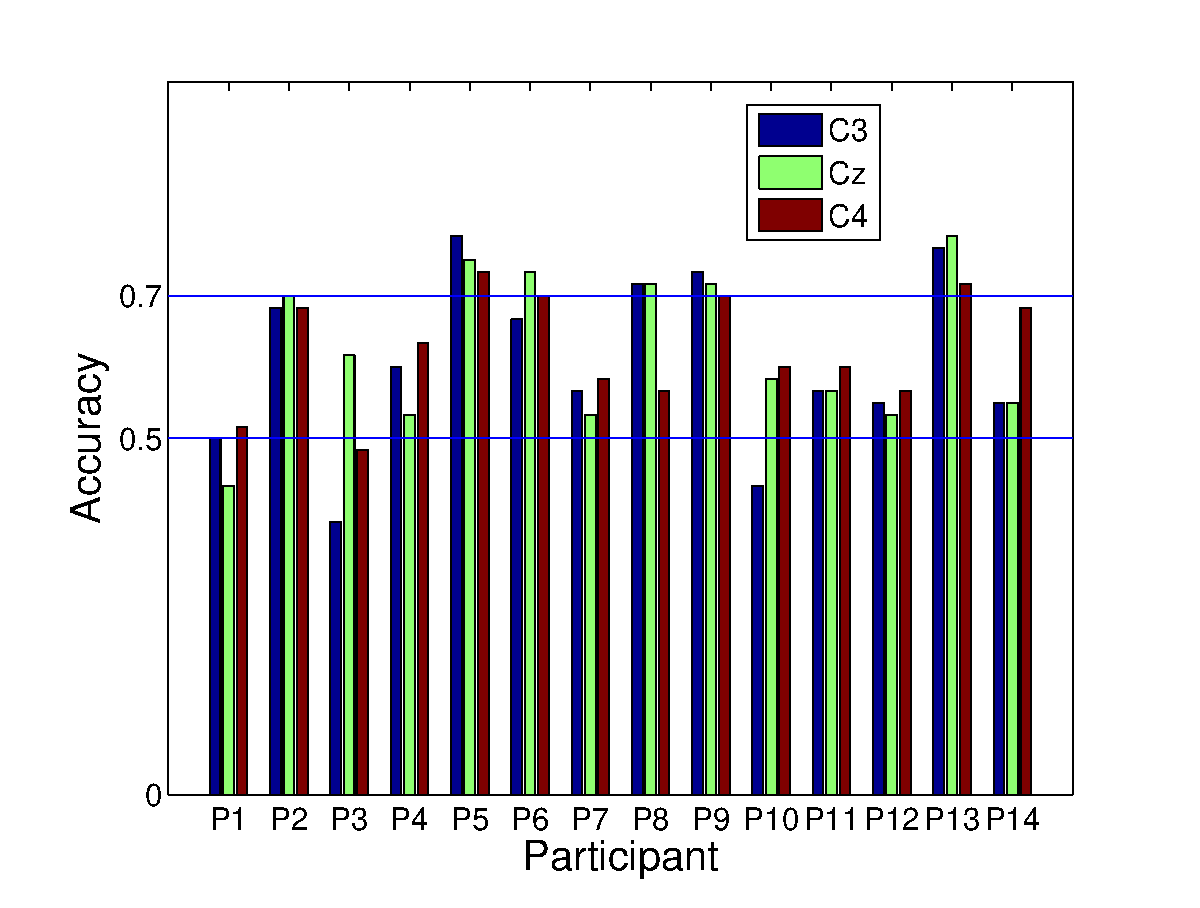
\includegraphics[scale=0.45]{images/DatasetMIBCISimulation2}}
      \caption{\centering Accuracy for the BCI Simulation classifying Baseline vs. FM (Feet Movement) motor imagery.}
      \label{figure3}
   \end{figure} 	
	\end{frame}	  
    
    \begin{frame}
   \begin{figure}[thpb]
      \centering
      \setlength\fboxsep{0pt}
	  \setlength\fboxrule{0.5pt}
       \fbox{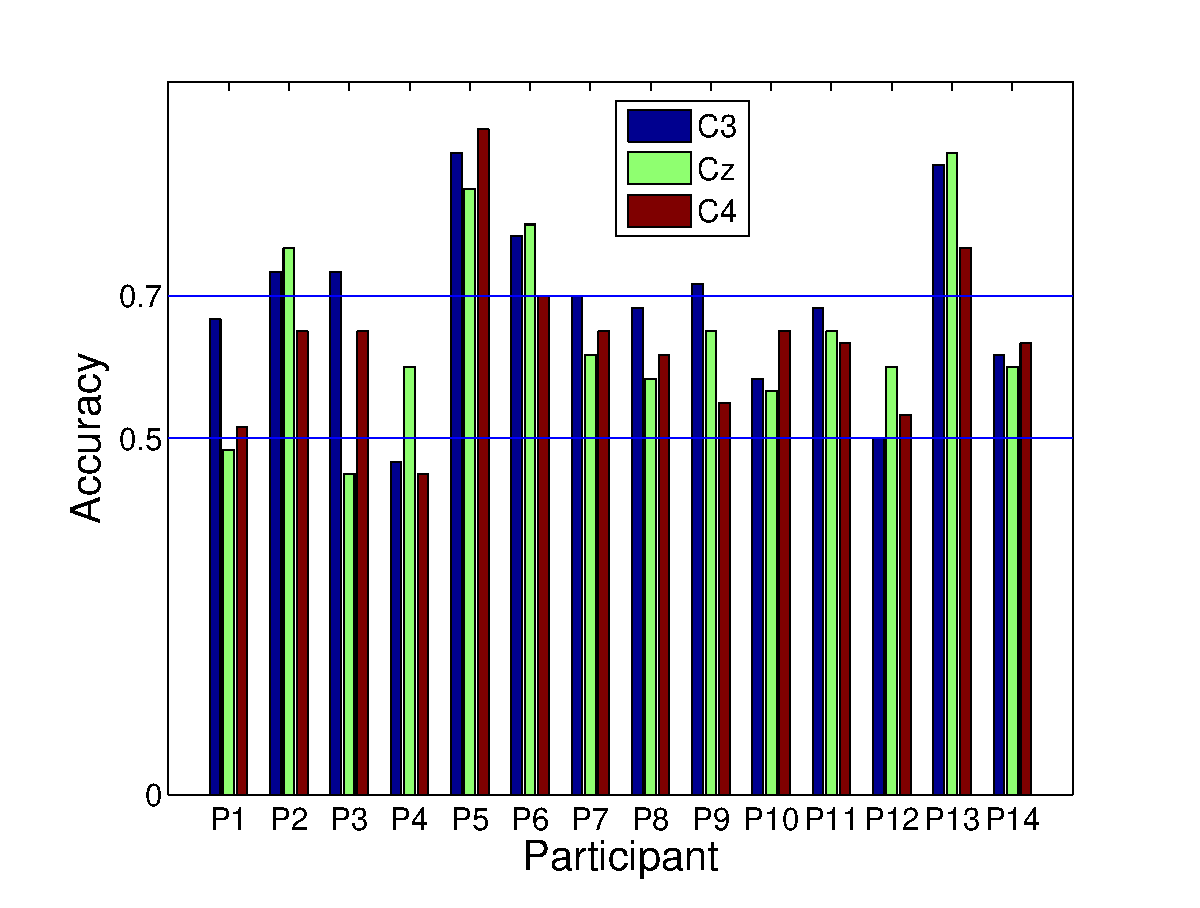
\includegraphics[scale=0.23]{images/DatasetMIBCISimulation1}}
       \fbox{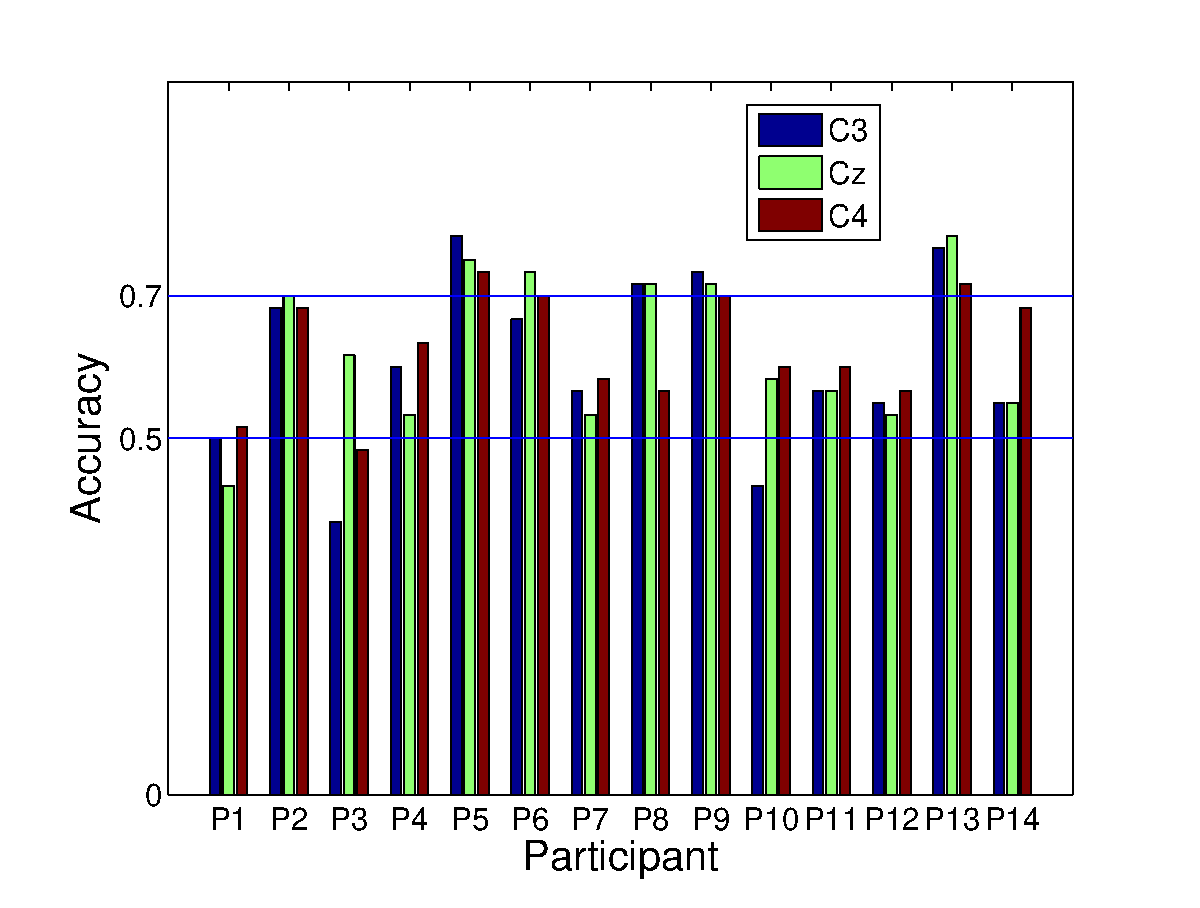
\includegraphics[scale=0.23]{images/DatasetMIBCISimulation2}}
      \caption{\centering Comparative results obtained for the Offline BCI Simulation using MI RH (left) and MI FM (right)}
      \label{figure3}
   \end{figure}  
    \end{frame}
    
    \section{Conclusion}
    \begin{frame}
        \frametitle{Conclusion}
        \begin{center}
            \begin{itemize}
                \item A method to analyze EEG signals was presented.
                \item A signal transformation algorithm was introduced.
                \item A classification scheme was implemented.
                \item Offline Alpha Waves presence was detected from signal plot with an accuracy level 10-fold cross validated of 70\%.
                \item Offline BCI Simulation of single trial asynchronous triggering for right hand MI based on signal plots was implemented with a level of success of 70\% for 7 out of 14 Participants. 
            \end{itemize}
        \end{center}
    \end{frame}    
    
    
    \section{References}
    \begin{frame} %Biblio
        \frametitle{References}
        \begin{itemize}
            \item Lowe 2004
			 \item Boiman, Shechtman, Irani 2008
			 \item Ramele, Villar, Santos 2014
			 \item Goldberg et al 2000, Schalk 2004
			 \item Steyrl, Scherer et al 2015
        \end{itemize}
    \end{frame}


\end{document}